\documentclass{beamer}
\usepackage[spanish]{babel}
\usepackage[utf8]{inputenc}
\usepackage{lmodern} % para cualquier tamaño de letra
\usepackage{amsmath}
\usepackage{amsfonts}
\usetheme{Copenhagen}
\setbeamercovered{transparent=30}

\begin{document}

\title{Compresión JPEG}
\author{Balbi Pablo Luis, Pazos Méndez Nicolás Javier}
\date{\today}

\begin{frame}
    \titlepage
\end{frame}

\begin{frame}
    \frametitle{Cómo viene la cosa...}
    \tableofcontents[hideallsubsections]
\end{frame}

\section{El método de compresión JPEG}
\begin{frame}
    \frametitle{El método de compresión JPEG}
        Cuatro pasos fundamentales:
        [NOTE]: Quedrá muy choto aca hacer un dibujito de pipeline a mano, escanearlo y ponerlo?
        tipo este \url{https://m.eet.com/media/1101219/fig1.jpg}
        \begin{enumerate}
            \item Separar la imagen en cuadrados de $8 \times 8$
            \item Aplicar la DCT\footnote{transformada del coseno discreta} a cada cuadrado
            \item Cuantizar los coeficientes del paso anterior
            \item Comprimir el conjunto de coeficientes finales
        \end{enumerate}

\end{frame}

\begin{frame}
    \frametitle{DCT}
    \begin{center}
        Una imagen $I$ de $NM$ pixels, es una matriz en $A^{NM}$, con $A = \{x \in \mathbb{N} \text{ si
        $0 \leq x \leq 255$}\}$ \vspace{6mm}

        La DCT tiene la siguiente ecuación:\vspace{6mm}

        $F(u,v)=\frac{1}{NM}C(u)C(v)\,\sum_{x=0}^{7} \sum_{y=0}^{7}\,I(x,y)\,B(u,v,x,y)$

        \vspace{3mm} 
        $f(x,y)=\frac{1}{NM}\,\sum_{x=0}^{7} \sum_{y=0}^{7}\,C(u)C(v)\,F(u,v)\,B(u,v,x,y)$

        \vspace{3mm}
        donde
        \vspace{3mm}

        $B(u,v,x,y) = cos\frac{(2x+1)u\pi}{16}cos\frac{(2y+1)v\pi}{16}$
        \[   
        C(j) = 
             \begin{cases}
                 \frac{1}{\sqrt{2}}\text{ si $j=0$}\\
                 1 \text{ sino}\\
             \end{cases}
        \]
        NOTE: Quizas meter aca un "si la comparamos con la DFT no es tan diferente, escribiendo
        ambas"
    \end{center}
\end{frame}

\begin{frame}
    \frametitle{Separar la imagen en cuadrados de $8 \times 8$}
    \begin{minipage}[t]{0.48\linewidth}
        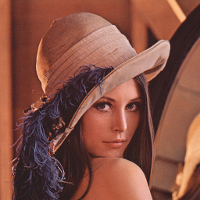
\includegraphics[width=5cm, height=5cm]{fig/lena.png}
    \end{minipage}
    \hfill
    \begin{minipage}[t]{0.48\linewidth}
        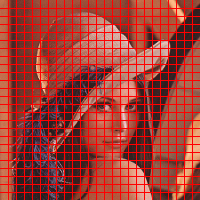
\includegraphics[width=5cm, height=5cm]{fig/lena_blocks.png}
    \end{minipage}
\end{frame}

\begin{frame}
    \frametitle{Separar la imagen en cuadrados de $8 \times 8$}
    \textbf{¿Por qué partir la imagen en bloques?}
    \begin{itemize}
        \item Aplicar la DCT a la imagen completa requiere más memoria y es menos modular. % sirve que sea modular para cosas tipo GPU
        \item Las imágenes no suelen ser completamente homogéneas. Analizar las frecuencias de la imagen completa no es lo mejor para comprimir.
    \end{itemize}
\end{frame}

\begin{frame}
    \frametitle{Separar la imagen en cuadrados de $8 \times 8$}
    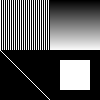
\includegraphics[width=5cm, height=5cm]{fig/no_homogenea.png}
\end{frame}

\begin{frame}
    \frametitle{Aplicar la DCT a cada cuadrado}
    [TODO] shifter -128 y aplicar la transformada

    [TODO] por qué usamos este espacio? porque las frecuencias bajas nos importan más

    [TODO] darles nombres a los coeficientes DC/AC para referirse después
\end{frame}

\begin{frame}
    \frametitle{Caracterizando un bloque}
    Un bloque es también una matriz $B \in A^{8x8}$

    \vspace{5mm}
    $B_{0,0}$
    

    
\end{frame}

\begin{frame}
    \frametitle{Cuantizar los coeficientes}
    [TODO] por qué cuantizamos? Para comprimir más y más fácil. bajamos la entropía.
    Es importante entender que no estamos descartando por frecuencias, sino
    que estamos estableciendo como un step.

    [TODO] cómo cuantizamos? Con la tabla de cuantización
\end{frame}

\begin{frame}
    \frametitle{Comprimir el conjunto de coeficientes finales}

    [TODO] ahora que bajamos mucho la entropía podemos comprimir mucho más. Pasos:
    \begin{enumerate}
        \item Codificar los coeficientes DC
        \item Desarmar en $zig-zag$ cada cuadrado
        \item Comprimir cada cuadrado como tuplas $(\# ceros \, antes, \, valor)$
        \item Codificar las tuplas con Huffman

    \end{enumerate}
\end{frame}
\begin{frame}
    \frametitle{ideas exps}
    \begin{itemize}
        \item Algo como esto: 
            \url{https://res.cloudinary.com/ddxwdqwkr/image/upload/q_100/v1502426282/essential-image-optimization/Modern-Image5.jpg}
    \end{itemize}
    
\end{frame}

\end{document}
